\hypertarget{location-sensors}{%
\section{Location Sensors}\label{location-sensors}}

\hypertarget{beacons}{%
\subsection{Beacons}\label{beacons}}

While IMUs are amazing devices, they cannot give us accurate position
information. Estimating the position in the environment is essential for
navigation. One approach is to instrument the environment. An example of
this would be placing markers that the robot sensors can detect and
reliably interpret for location information. We will explore several of
these ideas with beacon systems as our guiding example.

\texttt{Beacons} are probably the simplest approach to localization. A
beacon is any type of landmark with a known location. Natural beacons
such as stars, sun, moon, mountains, streams and other markers have been
used throughout human existence\footnote{One would assume that natural
  beacons are used by animals as well}. Manmade beacons include towers,
signs, lighthouses and other marked locations.

Indoor beacon systems include using colored or IR lights, RFID tags,
ultrasonic transducers, QR codes, colored tags and other forms of
environmental instrumentation. Normally this means that the environment
is modified in some detectable manner. Similar approaches can be done
outdoors, but since the introduction of GPS, it has dominated the
localization approaches. \texttt{GPS}, the
\texttt{Global\ Positioning\ System}, was developed for the US military
for their localization and navigation requirements.

GPS uses signals from satellites to triangulate position. Conceptually
it is rather simple to use time of flight from four satellites to
exactly locate an object. The challenges are that the distances are
great, the speed of light is very high and the Earth is often in the
way. To address the line of sight requirement, 24 satellites with
several spares orbit the earth every 12 hours at an altitude of 20,190
km. They are arranged as four satellites in six planes offset by 55
degrees from the plane of the equator. Knowing the time of flight and
the speed of light, distance of the observer from the satellite can be
determined.

There are several challenges to be overcome. First is a precise
measurement of the time of flight. Time synchronization between
satellites and GPS receiver is essential. Secondly, a precise location
of the satellite is required. In addition one needs to deal with signal
quality and interference.

\begin{quote}
Global Positioning System - GPS
\end{quote}

Each satellite has an atomic clock for ultra-precise tracking of time.
They are monitored by ground stations. These ground stations also track
the location of the satellites. The ground station can perform the
location analysis and transmit the position estimate to the satellites.

A GPS receiver will grab a code from the satellite which has time stamp
data. Using this information, the distance between the satellite and the
receiver is computed. The clock on most receivers is not very accurate
so information from more than three satellites are required to adjust
for local clock errors. This allows for estimates to be accurate within
several meters.

\begin{figure}
\centering
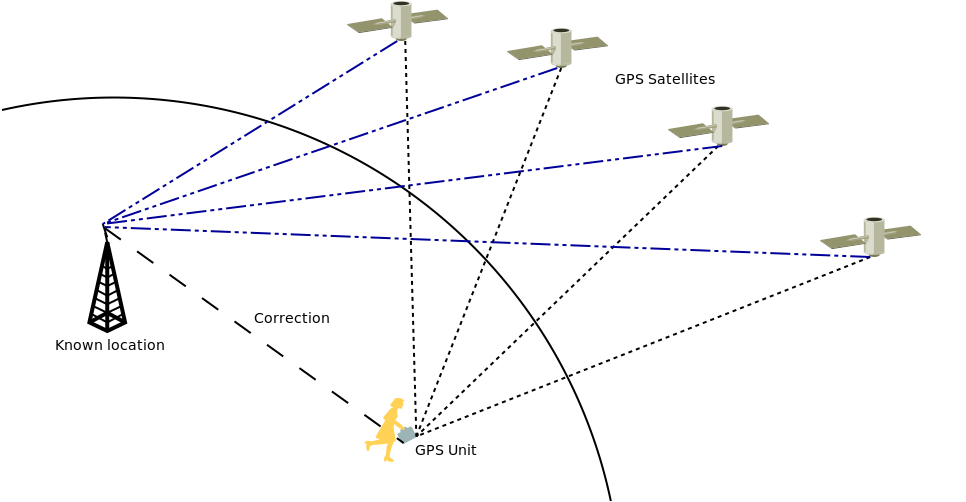
\includegraphics[width=0.5\textwidth,height=\textheight]{SensorsFigures/dgps.*}
\caption{GPS with local correction.}
\end{figure}

\hypertarget{example}{%
\subsubsection{Example}\label{example}}

Assume that you have four beacon towers located in roughly a square over
a 10km x 10km patch of land. You place a coordinate system on the land
and measure the beacon locations. The locations in meters are B1 (0,0),
B2 (56, 9752), B3 (9126, 7797), B4 (9863, 218). If the beacons transmit
a packet with a time stamp, then a mobile system with an accurate clock
can determine its location in the instrumented area. Determine locations
if \(t_1 = 22793\) ns, \(t_2 = 15930\) ns, \(t_3 = 20817\) ns,
\(t_4 =  29793\) ns. The distances are found via \(d = ct\):
\(d_1 = 6838 m\), \(d_2 = 4779 m\), \(d_3 = 6245 m\), \(d_4 = 8938 m\).
So our object lies on a circle of distance \(d_1\) from beacon one and
distance \(d_2\) from beacon two, etc.

One may intersect two circles to provide the location of the two
intersecting points and then proceed over all combinations:

\[(x-a_i)^2 + (y-b_i)^2 = r_i^2 , \quad (x-a_j)^2 + (y-b_j)^2 = r_j^2 .\]

The algebra can be simplified by expanding each circle equation

\[x^2 - 2a_ix + a_i^2 + y^2 - 2b_iy + b_i^2 = r_i^2 ,
\quad x^2 - 2a_jx + a_j^2 + y^2 - 2b_jy + b_j^2 = r_j^2\]

and computing a difference

\[2(a_j-a_i)x + 2(b_j-b_i)y + a_i^2-a_j^2 + b_i^2-b_j^2 = r_i^2 - r_j^2 .\]

Using three circle equations, you can obtain two linear equations

\[2(a_j-a_i)x + 2(b_j-b_i)y  = r_i^2 - r_j^2 - a_i^2 + a_j^2 - b_i^2 + b_j^2\]

\[2(a_k-a_i)x + 2(b_k-b_i)y = r_i^2 - r_k^2  - a_i^2 + a_k^2 - b_i^2  + b_k^2  .\]

In a noise free world, the solution would be where the circles intersect
exactly such as seen in \texttt{fig:exactintersection}. But this does
not happen due to noise and sensor inaccuracies. The circles do not
intersect as shown in \texttt{fig:inexactintersection}.

\begin{quote}
Exact intersection of three circles.

Non-intersection of three circles.
\end{quote}

One way to approach this problem is to cast into a optimization problem.
If we are a certain distance (in two dimensions) away from a beacon,
then we lie on a circle where the radius of the circle is the distance
away from the beacon. The object must lie on all of the circles which
are have the given distance.

We would like to minimize the distance that our selected point \((x,y)\)
lies off of each circle. The distance the point misses the circle from
B1 is \(|\sqrt{x^2 + y^2} - 6838|\). From the individual errors, we can
form the total error function by summing up the individual error terms.

\[\begin{aligned}
\begin{array}{ll}
E = & \quad  |\sqrt{x^2 + y^2} - 6838|
 + |\sqrt{(x-56)^2 + (y-9752)^2} - 4779|     \\[3mm]
& + |\sqrt{(x-9126)^2  + (y-7797)^2} - 6245|
 + |\sqrt{(x-9863)^2 + (y-218)^2} - 8938|  .
\end{array}
\end{aligned}\]

If \(E=0\), then we are at the \((x,y)\) point that matches all four
distances.

\begin{quote}
Radial error function.
\end{quote}

Since there is measurement error we will have in practice that
\(E > 0\), so we are looking for the minimum value for \(E\). A
traditional multivariate calculus approach is to take partial
derivatives and set them to zero. This produces a system of nonlinear
equations which must be solved numerically. It is the square root that
gives complicated algebra as well as division by zero errors.

One additional problem is the absolute value. The derivative of the
absolute \((d/dx) |x| = x /|x|\) is the sign function, \(sign(x)\) (not
\(\sin ()\)). This is not continuous and will wreak havoc on some
optimization codes. In addition, combinations of absolute values can
lead to non-single point minimums although unlikely in our case. To
address these issues, we change our error function by replacing the
absolute value with a square. Indeed this will change the function but
will allow for unique mins. Note that for a single component element of
the expression, \(|f(x,y)|\) the minimum will not move when we move to
\([f(x,y)]^2\). For sums, \(|f(x,y) + g(x,y)|\) this is no longer true,
but not necessarily a bad result.

There are several directions we can head to find the extremal. Many
variants of Newton's Method are available. One can imagine custom search
algorithms. For simplicity we will leave those approaches to text's on
numerical optimization and we will use gradient descent. Recall the
definition of the gradient is
\(\nabla E = \left< \partial E / \partial x, \partial E / \partial y \right>\).
The updated function to minimize is

\[\begin{aligned}
\begin{array}{ll}
E \quad = & \quad  \left(\sqrt{x^2 + y^2} - 6838\right)^2     \\[3mm]
 &+ \left(\sqrt{(x-56)^2 + (y-9752)^2} - 4779\right)^2    \\[3mm]
& + \left(\sqrt{(x-9126)^2  + (y-7797)^2} - 6245\right)^2   \\[3mm]
& + \left(\sqrt{(x-9863)^2 + (y-218)^2} - 8938\right)^2 .
\end{array}
\end{aligned}\]

Since we are using a numerical method (gradient descent) and thus not an
exact method, it makes sense to use a numerical approach to computing
the partial derivatives. Recall that the approximation of the derivative
is

\[\displaystyle \frac{\partial F}{\partial x_k} \approx \frac{F(x_1, x_2, \dots , x_k + \Delta x, \dots , x_n) - F(x_1, x_2, \dots  , x_n)}{\Delta x}\]

for small \(\Delta x\). For each item in the gradient vector, you can
estimate the derivative. This requires two function evaluations, a
difference and a multiply. {[}Precompute \(1/\Delta x\) and then
multiply.{]} For the algorithm, if you have rough guess as to location,
you can use this for your initial guess for gradient descent. Otherwise
you can pick the center or a random point in the search region.

\begin{description}
\item[We can use the gradient descent method to find the solution. Set]
\(x_0 = 5000\), \(y_0=5000\), \(k=0\), \(t=1\):
\end{description}

While (\(t > t_0\))

\begin{itemize}
\tightlist
\item
  \(u = \nabla E (x_k, y_k) /  \| \nabla E (x_k, y_k) \|\)
\item
  \((a,b) = (x_k,y_k) - t u\)
\item
  while \(\left[ E(a,b) > E(x_k,y_k)\right]\)

  \begin{itemize}
  \tightlist
  \item
    \(t = t/2\)
  \item
    \((a,b) = (x_k,y_k) - t u\)
  \end{itemize}
\item
  \(k=k+1\)
\item
  \((x_k,y_k) = (a,b)\)
\end{itemize}

\begin{verbatim}
function funct(x,y)
    E = (sqrt(x^2 + y^2) - 6838)^2 \
    + (sqrt((x-56)^2 + (y-9752)^2) - 4779)^2 \
    + (sqrt((x-9126)^2  + (y-7797)^2) - 6245)^2 \
    + (sqrt((x-9863)^2 + (y-218)^2) - 8938)^2
    return E
end
\end{verbatim}

\begin{verbatim}
# The numerical gradient approximation
function grad(x,y)
    delta = 0.0001
    E = funct(x,y)
    E1 = funct(x+delta,y)
    E2 = funct(x,y+delta)
    dEx = (E1-E)/delta
    dEy = (E2-E)/delta
    return dEx, dEy
end   
\end{verbatim}

\begin{verbatim}
# The size of the vector
function norm(r,s)
    return sqrt(r*r+s*s)
end

# The step in the direction (u,v)
function step(x,y, u,v,t)
    a = x - t*u
    b = y - t*v
    return a, b
end
\end{verbatim}

\begin{verbatim}
# Globals
x = 5000
y = 5000
t = 10.0
tsmall = 0.00001

# The descent algorithm
while (t > tsmall)
    global x, y, t
    dx, dy = grad(x,y)
    size = norm(dx,dy)
    u = dx/size
    v = dy/size
    a,b = step(x,y,u,v,t)
    while (funct(a,b) > funct(x,y))
        t = 0.5*t
        a,b = step(x,y,u,v,t)
    end
    x,y = a,b

end

println(x, "  ", y)
\end{verbatim}

\begin{Shaded}
\begin{Highlighting}[]
\CommentTok{\# The function definition}
\KeywordTok{function}\NormalTok{ funct(x}\OperatorTok{,}\NormalTok{y)}
\NormalTok{   E }\OperatorTok{=}\NormalTok{ (sqrt(x}\OperatorTok{\^{}}\FloatTok{2} \OperatorTok{+}\NormalTok{ y}\OperatorTok{\^{}}\FloatTok{2}\NormalTok{) }\OperatorTok{{-}} \FloatTok{6838}\NormalTok{)}\OperatorTok{\^{}}\FloatTok{2}  \OperatorTok{+}
\NormalTok{   (sqrt((x}\OperatorTok{{-}}\FloatTok{56}\NormalTok{)}\OperatorTok{\^{}}\FloatTok{2} \OperatorTok{+}\NormalTok{ (y}\OperatorTok{{-}}\FloatTok{9752}\NormalTok{)}\OperatorTok{\^{}}\FloatTok{2}\NormalTok{) }\OperatorTok{{-}} \FloatTok{4779}\NormalTok{)}\OperatorTok{\^{}}\FloatTok{2}  \OperatorTok{+}
\NormalTok{   (sqrt((x}\OperatorTok{{-}}\FloatTok{9126}\NormalTok{)}\OperatorTok{\^{}}\FloatTok{2}  \OperatorTok{+}\NormalTok{ (y}\OperatorTok{{-}}\FloatTok{7797}\NormalTok{)}\OperatorTok{\^{}}\FloatTok{2}\NormalTok{) }\OperatorTok{{-}} \FloatTok{6245}\NormalTok{)}\OperatorTok{\^{}}\FloatTok{2} \OperatorTok{+}
\NormalTok{   (sqrt((x}\OperatorTok{{-}}\FloatTok{9863}\NormalTok{)}\OperatorTok{\^{}}\FloatTok{2} \OperatorTok{+}\NormalTok{ (y}\OperatorTok{{-}}\FloatTok{218}\NormalTok{)}\OperatorTok{\^{}}\FloatTok{2}\NormalTok{) }\OperatorTok{{-}} \FloatTok{8938}\NormalTok{)}\OperatorTok{\^{}}\FloatTok{2}
   \KeywordTok{return}\NormalTok{ E}
\KeywordTok{end}
\end{Highlighting}
\end{Shaded}

\begin{Shaded}
\begin{Highlighting}[]
\CommentTok{\# The numerical gradient approximation}
\KeywordTok{function}\NormalTok{ grad(x}\OperatorTok{,}\NormalTok{y)}
\NormalTok{    delta }\OperatorTok{=} \FloatTok{0.0001}
\NormalTok{    E }\OperatorTok{=}\NormalTok{ funct(x}\OperatorTok{,}\NormalTok{y)}
\NormalTok{    E1 }\OperatorTok{=}\NormalTok{ funct(x}\OperatorTok{+}\NormalTok{delta}\OperatorTok{,}\NormalTok{y)}
\NormalTok{    E2 }\OperatorTok{=}\NormalTok{ funct(x}\OperatorTok{,}\NormalTok{y}\OperatorTok{+}\NormalTok{delta)}
\NormalTok{    dEx }\OperatorTok{=}\NormalTok{ (E1}\OperatorTok{{-}}\NormalTok{E)}\OperatorTok{/}\NormalTok{delta}
\NormalTok{    dEy }\OperatorTok{=}\NormalTok{ (E2}\OperatorTok{{-}}\NormalTok{E)}\OperatorTok{/}\NormalTok{delta}
    \KeywordTok{return}\NormalTok{ dEx}\OperatorTok{,}\NormalTok{ dEy}
\KeywordTok{end}
\end{Highlighting}
\end{Shaded}

\begin{Shaded}
\begin{Highlighting}[]
\CommentTok{\# The size of the vector}
\KeywordTok{function}\NormalTok{ norm(r}\OperatorTok{,}\NormalTok{s)}
    \KeywordTok{return}\NormalTok{ sqrt(r}\OperatorTok{*}\NormalTok{r}\OperatorTok{+}\NormalTok{s}\OperatorTok{*}\NormalTok{s)}
\KeywordTok{end}

\CommentTok{\# The step in the direction (u,v)}
\KeywordTok{function}\NormalTok{ step(x}\OperatorTok{,}\NormalTok{y}\OperatorTok{,}\NormalTok{ u}\OperatorTok{,}\NormalTok{v}\OperatorTok{,}\NormalTok{t)}
\NormalTok{    a }\OperatorTok{=}\NormalTok{ x }\OperatorTok{{-}}\NormalTok{ t}\OperatorTok{*}\NormalTok{u}
\NormalTok{    b }\OperatorTok{=}\NormalTok{ y }\OperatorTok{{-}}\NormalTok{ t}\OperatorTok{*}\NormalTok{v}
    \KeywordTok{return}\NormalTok{ a}\OperatorTok{,}\NormalTok{ b}
\KeywordTok{end}  
\end{Highlighting}
\end{Shaded}

\begin{Shaded}
\begin{Highlighting}[]
\CommentTok{\# Globals}
\NormalTok{x }\OperatorTok{=} \FloatTok{5000}
\NormalTok{y }\OperatorTok{=} \FloatTok{5000}
\NormalTok{t }\OperatorTok{=} \FloatTok{10.0}
\NormalTok{tsmall }\OperatorTok{=} \FloatTok{0.00001}

\CommentTok{\# The descent algorithm}
\KeywordTok{while}\NormalTok{ (t }\OperatorTok{\textgreater{}}\NormalTok{ tsmall)}
\NormalTok{    dx}\OperatorTok{,}\NormalTok{ dy }\OperatorTok{=}\NormalTok{ grad(x}\OperatorTok{,}\NormalTok{y)}
\NormalTok{    size }\OperatorTok{=}\NormalTok{ norm(dx}\OperatorTok{,}\NormalTok{dy)}
\NormalTok{    u }\OperatorTok{=}\NormalTok{ dx}\OperatorTok{/}\NormalTok{size}
\NormalTok{    v }\OperatorTok{=}\NormalTok{ dy}\OperatorTok{/}\NormalTok{size}
\NormalTok{    a}\OperatorTok{,}\NormalTok{b }\OperatorTok{=}\NormalTok{ step(x}\OperatorTok{,}\NormalTok{y}\OperatorTok{,}\NormalTok{u}\OperatorTok{,}\NormalTok{v}\OperatorTok{,}\NormalTok{t)}
    \KeywordTok{while}\NormalTok{ (funct(a}\OperatorTok{,}\NormalTok{b) }\OperatorTok{\textgreater{}}\NormalTok{ funct(x}\OperatorTok{,}\NormalTok{y))}
\NormalTok{        t }\OperatorTok{=} \FloatTok{0.5}\OperatorTok{*}\NormalTok{t}
\NormalTok{        a}\OperatorTok{,}\NormalTok{b }\OperatorTok{=}\NormalTok{ step(x}\OperatorTok{,}\NormalTok{y}\OperatorTok{,}\NormalTok{u}\OperatorTok{,}\NormalTok{v}\OperatorTok{,}\NormalTok{t)}
    \KeywordTok{end}

\NormalTok{    x}\OperatorTok{,}\NormalTok{y }\OperatorTok{=}\NormalTok{ a}\OperatorTok{,}\NormalTok{b}
\KeywordTok{end}

\NormalTok{println(}\StringTok{"x: "}\OperatorTok{,}\NormalTok{ x}\OperatorTok{,} \StringTok{" y: "}\OperatorTok{,}\NormalTok{ y)}
\end{Highlighting}
\end{Shaded}

\begin{figure}
\centering
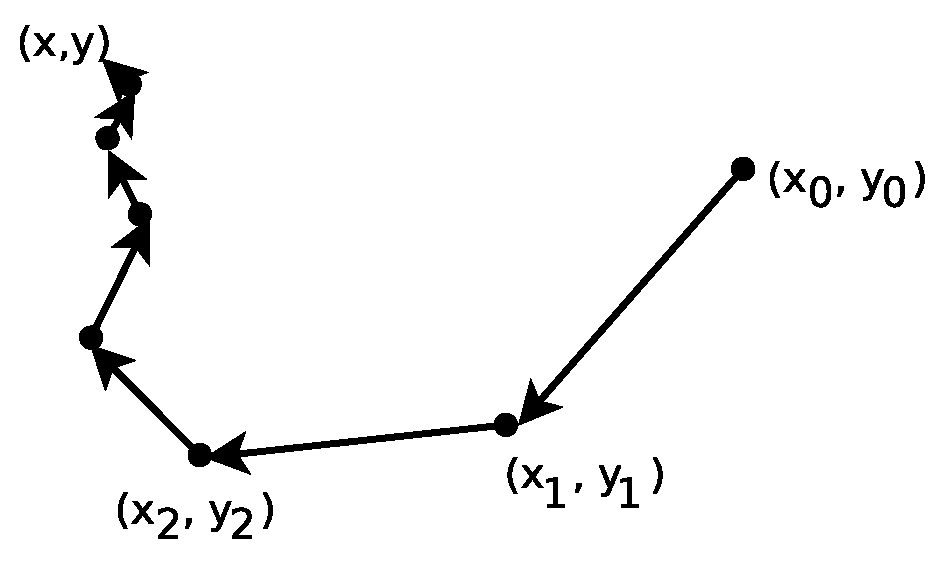
\includegraphics[width=0.5\textwidth,height=\textheight]{SensorsFigures/graddescent.*}
\caption{Gradient Descent}
\end{figure}

The intersection point is \(x = 3120\), \(y = 6085\). Note that this
algorithm is not guaranteed to converge on the solution (the global
minimum). It can get trapped in local minima. To address this problem
you may re-run the algorithm with different random starting points.

There are plenty of other ways to treat this problem. An image
processing approach akin to the Hough Transform (with voting) would also
work. It is also possible to lay down a grid and then increment grid
cells for each circle that passes through. The cell with the largest
value is a candidate for the location. Starting with a course grid and
refining the grid is a way to produce a hierarchal method that can have
high accuracy but still be fast. See if you can come up with other
approaches to this example.

\begin{figure}
\centering
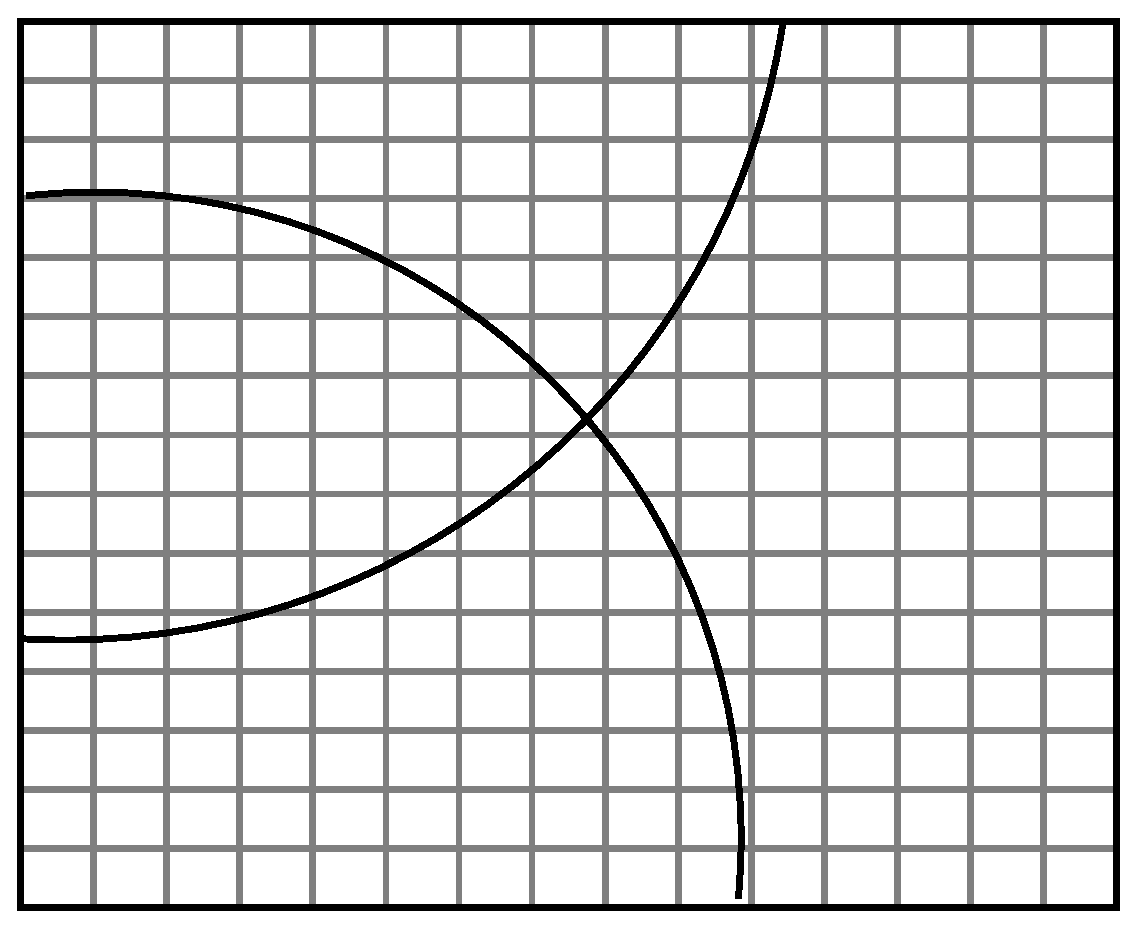
\includegraphics[width=0.5\textwidth,height=\textheight]{SensorsFigures/hough.*}
\caption{Hough Transform}
\end{figure}

\textbf{Footnote}
